\documentclass[tikz,border=10pt]{standalone}
\usepackage{tikz}
\usetikzlibrary{calc}

\begin{document}
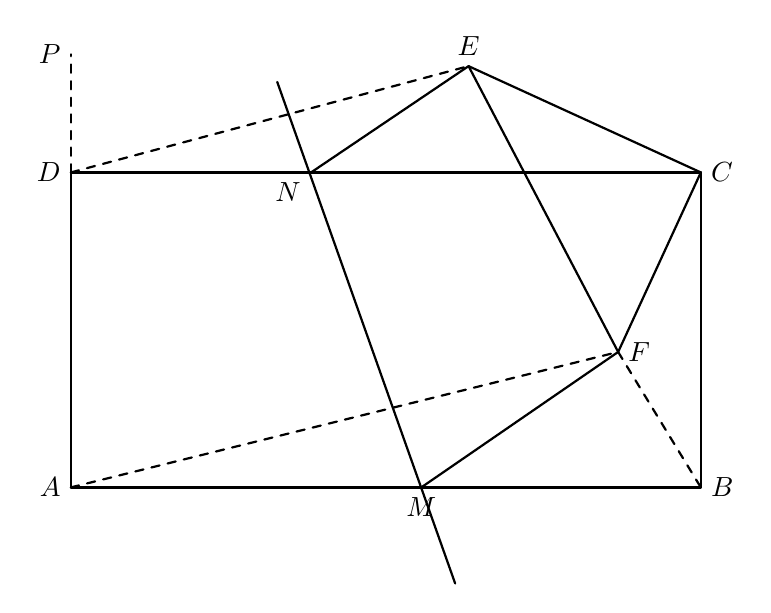
\begin{tikzpicture}[line cap=round,line join=round,thick]

% Coordinates
\coordinate (A) at (0,0);
\coordinate (B) at (8,0);
\coordinate (C) at (8,4);
\coordinate (D) at (0,4);
\coordinate (P) at (0,5.5);

\coordinate (M) at (4.45,0);
\coordinate (N) at (3.05,4);
\coordinate (E) at (5.05,5.35);
\coordinate (F) at (6.95,1.72);

% an extra point to define the slanted line through N and M
\coordinate (Q) at (2.62,5.15);
\coordinate (R) at (4.88,-1.22);

% Outer rectangle-like frame
\draw (A) -- (B);
\draw (B) -- (C);
\draw (D) -- (C);
\draw (A) -- (D);

% Dashed extensions and hidden segments
\draw[dashed] (D) -- (P);
\draw[dashed] (D) -- (E);
\draw[dashed] (A) -- (F);
\draw[dashed] (F) -- (B);

% Slanted line through N and M
\draw (Q) -- (R);

% Inner polygonal figure
\draw (N) -- (E) -- (C);
\draw (E) -- (F);
\draw (F) -- (C);
\draw (M) -- (F);

% Labels
\node[left] at (A) {$A$};
\node[right] at (B) {$B$};
\node[right] at (C) {$C$};
\node[left] at (D) {$D$};
\node[left] at (P) {$P$};

\node[below] at (M) {$M$};
\node[below left] at (N) {$N$};
\node[above] at (E) {$E$};
\node[right] at (F) {$F$};

\end{tikzpicture}
\end{document}
